
% Default to the notebook output style

    


% Inherit from the specified cell style.




    
\documentclass[11pt]{article}
\usepackage{float}
   \author{Collin Heist}
    
    \usepackage[T1]{fontenc}
    % Nicer default font (+ math font) than Computer Modern for most use cases
    \usepackage{mathpazo}

    % Basic figure setup, for now with no caption control since it's done
    % automatically by Pandoc (which extracts ![](path) syntax from Markdown).
    \usepackage{graphicx}
    % We will generate all images so they have a width \maxwidth. This means
    % that they will get their normal width if they fit onto the page, but
    % are scaled down if they would overflow the margins.
    \makeatletter
    \def\maxwidth{\ifdim\Gin@nat@width>\linewidth\linewidth
    \else\Gin@nat@width\fi}
    \makeatother
    \let\Oldincludegraphics\includegraphics
    % Set max figure width to be 80% of text width, for now hardcoded.
    \renewcommand{\includegraphics}[1]{\Oldincludegraphics[width=.8\maxwidth]{#1}}
    % Ensure that by default, figures have no caption (until we provide a
    % proper Figure object with a Caption API and a way to capture that
    % in the conversion process - todo).
    \usepackage{caption}
    \DeclareCaptionLabelFormat{nolabel}{}
    \captionsetup{labelformat=nolabel}

    \usepackage{adjustbox} % Used to constrain images to a maximum size 
    \usepackage{xcolor} % Allow colors to be defined
    \usepackage{enumerate} % Needed for markdown enumerations to work
    \usepackage{geometry} % Used to adjust the document margins
    \usepackage{amsmath} % Equations
    \usepackage{amssymb} % Equations
    \usepackage{textcomp} % defines textquotesingle
    % Hack from http://tex.stackexchange.com/a/47451/13684:
    \AtBeginDocument{%
        \def\PYZsq{\textquotesingle}% Upright quotes in Pygmentized code
    }
    \usepackage{upquote} % Upright quotes for verbatim code
    \usepackage{eurosym} % defines \euro
    \usepackage[mathletters]{ucs} % Extended unicode (utf-8) support
    \usepackage[utf8x]{inputenc} % Allow utf-8 characters in the tex document
    \usepackage{fancyvrb} % verbatim replacement that allows latex
    \usepackage{grffile} % extends the file name processing of package graphics 
                         % to support a larger range 
    % The hyperref package gives us a pdf with properly built
    % internal navigation ('pdf bookmarks' for the table of contents,
    % internal cross-reference links, web links for URLs, etc.)
    \usepackage{hyperref}
    \usepackage{longtable} % longtable support required by pandoc >1.10
    \usepackage{booktabs}  % table support for pandoc > 1.12.2
    \usepackage[inline]{enumitem} % IRkernel/repr support (it uses the enumerate* environment)
    \usepackage[normalem]{ulem} % ulem is needed to support strikethroughs (\sout)
                                % normalem makes italics be italics, not underlines
    \usepackage{mathrsfs}
    

    
    
    % Colors for the hyperref package
    \definecolor{urlcolor}{rgb}{0,.145,.698}
    \definecolor{linkcolor}{rgb}{.71,0.21,0.01}
    \definecolor{citecolor}{rgb}{.12,.54,.11}

    % ANSI colors
    \definecolor{ansi-black}{HTML}{3E424D}
    \definecolor{ansi-black-intense}{HTML}{282C36}
    \definecolor{ansi-red}{HTML}{E75C58}
    \definecolor{ansi-red-intense}{HTML}{B22B31}
    \definecolor{ansi-green}{HTML}{00A250}
    \definecolor{ansi-green-intense}{HTML}{007427}
    \definecolor{ansi-yellow}{HTML}{DDB62B}
    \definecolor{ansi-yellow-intense}{HTML}{B27D12}
    \definecolor{ansi-blue}{HTML}{208FFB}
    \definecolor{ansi-blue-intense}{HTML}{0065CA}
    \definecolor{ansi-magenta}{HTML}{D160C4}
    \definecolor{ansi-magenta-intense}{HTML}{A03196}
    \definecolor{ansi-cyan}{HTML}{60C6C8}
    \definecolor{ansi-cyan-intense}{HTML}{258F8F}
    \definecolor{ansi-white}{HTML}{C5C1B4}
    \definecolor{ansi-white-intense}{HTML}{A1A6B2}
    \definecolor{ansi-default-inverse-fg}{HTML}{FFFFFF}
    \definecolor{ansi-default-inverse-bg}{HTML}{000000}

    % commands and environments needed by pandoc snippets
    % extracted from the output of `pandoc -s`
    \providecommand{\tightlist}{%
      \setlength{\itemsep}{0pt}\setlength{\parskip}{0pt}}
    \DefineVerbatimEnvironment{Highlighting}{Verbatim}{commandchars=\\\{\}}
    % Add ',fontsize=\small' for more characters per line
    \newenvironment{Shaded}{}{}
    \newcommand{\KeywordTok}[1]{\textcolor[rgb]{0.00,0.44,0.13}{\textbf{{#1}}}}
    \newcommand{\DataTypeTok}[1]{\textcolor[rgb]{0.56,0.13,0.00}{{#1}}}
    \newcommand{\DecValTok}[1]{\textcolor[rgb]{0.25,0.63,0.44}{{#1}}}
    \newcommand{\BaseNTok}[1]{\textcolor[rgb]{0.25,0.63,0.44}{{#1}}}
    \newcommand{\FloatTok}[1]{\textcolor[rgb]{0.25,0.63,0.44}{{#1}}}
    \newcommand{\CharTok}[1]{\textcolor[rgb]{0.25,0.44,0.63}{{#1}}}
    \newcommand{\StringTok}[1]{\textcolor[rgb]{0.25,0.44,0.63}{{#1}}}
    \newcommand{\CommentTok}[1]{\textcolor[rgb]{0.38,0.63,0.69}{\textit{{#1}}}}
    \newcommand{\OtherTok}[1]{\textcolor[rgb]{0.00,0.44,0.13}{{#1}}}
    \newcommand{\AlertTok}[1]{\textcolor[rgb]{1.00,0.00,0.00}{\textbf{{#1}}}}
    \newcommand{\FunctionTok}[1]{\textcolor[rgb]{0.02,0.16,0.49}{{#1}}}
    \newcommand{\RegionMarkerTok}[1]{{#1}}
    \newcommand{\ErrorTok}[1]{\textcolor[rgb]{1.00,0.00,0.00}{\textbf{{#1}}}}
    \newcommand{\NormalTok}[1]{{#1}}
    
    % Additional commands for more recent versions of Pandoc
    \newcommand{\ConstantTok}[1]{\textcolor[rgb]{0.53,0.00,0.00}{{#1}}}
    \newcommand{\SpecialCharTok}[1]{\textcolor[rgb]{0.25,0.44,0.63}{{#1}}}
    \newcommand{\VerbatimStringTok}[1]{\textcolor[rgb]{0.25,0.44,0.63}{{#1}}}
    \newcommand{\SpecialStringTok}[1]{\textcolor[rgb]{0.73,0.40,0.53}{{#1}}}
    \newcommand{\ImportTok}[1]{{#1}}
    \newcommand{\DocumentationTok}[1]{\textcolor[rgb]{0.73,0.13,0.13}{\textit{{#1}}}}
    \newcommand{\AnnotationTok}[1]{\textcolor[rgb]{0.38,0.63,0.69}{\textbf{\textit{{#1}}}}}
    \newcommand{\CommentVarTok}[1]{\textcolor[rgb]{0.38,0.63,0.69}{\textbf{\textit{{#1}}}}}
    \newcommand{\VariableTok}[1]{\textcolor[rgb]{0.10,0.09,0.49}{{#1}}}
    \newcommand{\ControlFlowTok}[1]{\textcolor[rgb]{0.00,0.44,0.13}{\textbf{{#1}}}}
    \newcommand{\OperatorTok}[1]{\textcolor[rgb]{0.40,0.40,0.40}{{#1}}}
    \newcommand{\BuiltInTok}[1]{{#1}}
    \newcommand{\ExtensionTok}[1]{{#1}}
    \newcommand{\PreprocessorTok}[1]{\textcolor[rgb]{0.74,0.48,0.00}{{#1}}}
    \newcommand{\AttributeTok}[1]{\textcolor[rgb]{0.49,0.56,0.16}{{#1}}}
    \newcommand{\InformationTok}[1]{\textcolor[rgb]{0.38,0.63,0.69}{\textbf{\textit{{#1}}}}}
    \newcommand{\WarningTok}[1]{\textcolor[rgb]{0.38,0.63,0.69}{\textbf{\textit{{#1}}}}}
    
    
    % Define a nice break command that doesn't care if a line doesn't already
    % exist.
    \def\br{\hspace*{\fill} \\* }
    % Math Jax compatibility definitions
    \def\gt{>}
    \def\lt{<}
    \let\Oldtex\TeX
    \let\Oldlatex\LaTeX
    \renewcommand{\TeX}{\textrm{\Oldtex}}
    \renewcommand{\LaTeX}{\textrm{\Oldlatex}}
    % Document parameters
    % Document title
    \title{ECE 351 - Final Project}
    
    
    
    
    

    % Pygments definitions
    
\makeatletter
\def\PY@reset{\let\PY@it=\relax \let\PY@bf=\relax%
    \let\PY@ul=\relax \let\PY@tc=\relax%
    \let\PY@bc=\relax \let\PY@ff=\relax}
\def\PY@tok#1{\csname PY@tok@#1\endcsname}
\def\PY@toks#1+{\ifx\relax#1\empty\else%
    \PY@tok{#1}\expandafter\PY@toks\fi}
\def\PY@do#1{\PY@bc{\PY@tc{\PY@ul{%
    \PY@it{\PY@bf{\PY@ff{#1}}}}}}}
\def\PY#1#2{\PY@reset\PY@toks#1+\relax+\PY@do{#2}}

\expandafter\def\csname PY@tok@w\endcsname{\def\PY@tc##1{\textcolor[rgb]{0.73,0.73,0.73}{##1}}}
\expandafter\def\csname PY@tok@c\endcsname{\let\PY@it=\textit\def\PY@tc##1{\textcolor[rgb]{0.25,0.50,0.50}{##1}}}
\expandafter\def\csname PY@tok@cp\endcsname{\def\PY@tc##1{\textcolor[rgb]{0.74,0.48,0.00}{##1}}}
\expandafter\def\csname PY@tok@k\endcsname{\let\PY@bf=\textbf\def\PY@tc##1{\textcolor[rgb]{0.00,0.50,0.00}{##1}}}
\expandafter\def\csname PY@tok@kp\endcsname{\def\PY@tc##1{\textcolor[rgb]{0.00,0.50,0.00}{##1}}}
\expandafter\def\csname PY@tok@kt\endcsname{\def\PY@tc##1{\textcolor[rgb]{0.69,0.00,0.25}{##1}}}
\expandafter\def\csname PY@tok@o\endcsname{\def\PY@tc##1{\textcolor[rgb]{0.40,0.40,0.40}{##1}}}
\expandafter\def\csname PY@tok@ow\endcsname{\let\PY@bf=\textbf\def\PY@tc##1{\textcolor[rgb]{0.67,0.13,1.00}{##1}}}
\expandafter\def\csname PY@tok@nb\endcsname{\def\PY@tc##1{\textcolor[rgb]{0.00,0.50,0.00}{##1}}}
\expandafter\def\csname PY@tok@nf\endcsname{\def\PY@tc##1{\textcolor[rgb]{0.00,0.00,1.00}{##1}}}
\expandafter\def\csname PY@tok@nc\endcsname{\let\PY@bf=\textbf\def\PY@tc##1{\textcolor[rgb]{0.00,0.00,1.00}{##1}}}
\expandafter\def\csname PY@tok@nn\endcsname{\let\PY@bf=\textbf\def\PY@tc##1{\textcolor[rgb]{0.00,0.00,1.00}{##1}}}
\expandafter\def\csname PY@tok@ne\endcsname{\let\PY@bf=\textbf\def\PY@tc##1{\textcolor[rgb]{0.82,0.25,0.23}{##1}}}
\expandafter\def\csname PY@tok@nv\endcsname{\def\PY@tc##1{\textcolor[rgb]{0.10,0.09,0.49}{##1}}}
\expandafter\def\csname PY@tok@no\endcsname{\def\PY@tc##1{\textcolor[rgb]{0.53,0.00,0.00}{##1}}}
\expandafter\def\csname PY@tok@nl\endcsname{\def\PY@tc##1{\textcolor[rgb]{0.63,0.63,0.00}{##1}}}
\expandafter\def\csname PY@tok@ni\endcsname{\let\PY@bf=\textbf\def\PY@tc##1{\textcolor[rgb]{0.60,0.60,0.60}{##1}}}
\expandafter\def\csname PY@tok@na\endcsname{\def\PY@tc##1{\textcolor[rgb]{0.49,0.56,0.16}{##1}}}
\expandafter\def\csname PY@tok@nt\endcsname{\let\PY@bf=\textbf\def\PY@tc##1{\textcolor[rgb]{0.00,0.50,0.00}{##1}}}
\expandafter\def\csname PY@tok@nd\endcsname{\def\PY@tc##1{\textcolor[rgb]{0.67,0.13,1.00}{##1}}}
\expandafter\def\csname PY@tok@s\endcsname{\def\PY@tc##1{\textcolor[rgb]{0.73,0.13,0.13}{##1}}}
\expandafter\def\csname PY@tok@sd\endcsname{\let\PY@it=\textit\def\PY@tc##1{\textcolor[rgb]{0.73,0.13,0.13}{##1}}}
\expandafter\def\csname PY@tok@si\endcsname{\let\PY@bf=\textbf\def\PY@tc##1{\textcolor[rgb]{0.73,0.40,0.53}{##1}}}
\expandafter\def\csname PY@tok@se\endcsname{\let\PY@bf=\textbf\def\PY@tc##1{\textcolor[rgb]{0.73,0.40,0.13}{##1}}}
\expandafter\def\csname PY@tok@sr\endcsname{\def\PY@tc##1{\textcolor[rgb]{0.73,0.40,0.53}{##1}}}
\expandafter\def\csname PY@tok@ss\endcsname{\def\PY@tc##1{\textcolor[rgb]{0.10,0.09,0.49}{##1}}}
\expandafter\def\csname PY@tok@sx\endcsname{\def\PY@tc##1{\textcolor[rgb]{0.00,0.50,0.00}{##1}}}
\expandafter\def\csname PY@tok@m\endcsname{\def\PY@tc##1{\textcolor[rgb]{0.40,0.40,0.40}{##1}}}
\expandafter\def\csname PY@tok@gh\endcsname{\let\PY@bf=\textbf\def\PY@tc##1{\textcolor[rgb]{0.00,0.00,0.50}{##1}}}
\expandafter\def\csname PY@tok@gu\endcsname{\let\PY@bf=\textbf\def\PY@tc##1{\textcolor[rgb]{0.50,0.00,0.50}{##1}}}
\expandafter\def\csname PY@tok@gd\endcsname{\def\PY@tc##1{\textcolor[rgb]{0.63,0.00,0.00}{##1}}}
\expandafter\def\csname PY@tok@gi\endcsname{\def\PY@tc##1{\textcolor[rgb]{0.00,0.63,0.00}{##1}}}
\expandafter\def\csname PY@tok@gr\endcsname{\def\PY@tc##1{\textcolor[rgb]{1.00,0.00,0.00}{##1}}}
\expandafter\def\csname PY@tok@ge\endcsname{\let\PY@it=\textit}
\expandafter\def\csname PY@tok@gs\endcsname{\let\PY@bf=\textbf}
\expandafter\def\csname PY@tok@gp\endcsname{\let\PY@bf=\textbf\def\PY@tc##1{\textcolor[rgb]{0.00,0.00,0.50}{##1}}}
\expandafter\def\csname PY@tok@go\endcsname{\def\PY@tc##1{\textcolor[rgb]{0.53,0.53,0.53}{##1}}}
\expandafter\def\csname PY@tok@gt\endcsname{\def\PY@tc##1{\textcolor[rgb]{0.00,0.27,0.87}{##1}}}
\expandafter\def\csname PY@tok@err\endcsname{\def\PY@bc##1{\setlength{\fboxsep}{0pt}\fcolorbox[rgb]{1.00,0.00,0.00}{1,1,1}{\strut ##1}}}
\expandafter\def\csname PY@tok@kc\endcsname{\let\PY@bf=\textbf\def\PY@tc##1{\textcolor[rgb]{0.00,0.50,0.00}{##1}}}
\expandafter\def\csname PY@tok@kd\endcsname{\let\PY@bf=\textbf\def\PY@tc##1{\textcolor[rgb]{0.00,0.50,0.00}{##1}}}
\expandafter\def\csname PY@tok@kn\endcsname{\let\PY@bf=\textbf\def\PY@tc##1{\textcolor[rgb]{0.00,0.50,0.00}{##1}}}
\expandafter\def\csname PY@tok@kr\endcsname{\let\PY@bf=\textbf\def\PY@tc##1{\textcolor[rgb]{0.00,0.50,0.00}{##1}}}
\expandafter\def\csname PY@tok@bp\endcsname{\def\PY@tc##1{\textcolor[rgb]{0.00,0.50,0.00}{##1}}}
\expandafter\def\csname PY@tok@fm\endcsname{\def\PY@tc##1{\textcolor[rgb]{0.00,0.00,1.00}{##1}}}
\expandafter\def\csname PY@tok@vc\endcsname{\def\PY@tc##1{\textcolor[rgb]{0.10,0.09,0.49}{##1}}}
\expandafter\def\csname PY@tok@vg\endcsname{\def\PY@tc##1{\textcolor[rgb]{0.10,0.09,0.49}{##1}}}
\expandafter\def\csname PY@tok@vi\endcsname{\def\PY@tc##1{\textcolor[rgb]{0.10,0.09,0.49}{##1}}}
\expandafter\def\csname PY@tok@vm\endcsname{\def\PY@tc##1{\textcolor[rgb]{0.10,0.09,0.49}{##1}}}
\expandafter\def\csname PY@tok@sa\endcsname{\def\PY@tc##1{\textcolor[rgb]{0.73,0.13,0.13}{##1}}}
\expandafter\def\csname PY@tok@sb\endcsname{\def\PY@tc##1{\textcolor[rgb]{0.73,0.13,0.13}{##1}}}
\expandafter\def\csname PY@tok@sc\endcsname{\def\PY@tc##1{\textcolor[rgb]{0.73,0.13,0.13}{##1}}}
\expandafter\def\csname PY@tok@dl\endcsname{\def\PY@tc##1{\textcolor[rgb]{0.73,0.13,0.13}{##1}}}
\expandafter\def\csname PY@tok@s2\endcsname{\def\PY@tc##1{\textcolor[rgb]{0.73,0.13,0.13}{##1}}}
\expandafter\def\csname PY@tok@sh\endcsname{\def\PY@tc##1{\textcolor[rgb]{0.73,0.13,0.13}{##1}}}
\expandafter\def\csname PY@tok@s1\endcsname{\def\PY@tc##1{\textcolor[rgb]{0.73,0.13,0.13}{##1}}}
\expandafter\def\csname PY@tok@mb\endcsname{\def\PY@tc##1{\textcolor[rgb]{0.40,0.40,0.40}{##1}}}
\expandafter\def\csname PY@tok@mf\endcsname{\def\PY@tc##1{\textcolor[rgb]{0.40,0.40,0.40}{##1}}}
\expandafter\def\csname PY@tok@mh\endcsname{\def\PY@tc##1{\textcolor[rgb]{0.40,0.40,0.40}{##1}}}
\expandafter\def\csname PY@tok@mi\endcsname{\def\PY@tc##1{\textcolor[rgb]{0.40,0.40,0.40}{##1}}}
\expandafter\def\csname PY@tok@il\endcsname{\def\PY@tc##1{\textcolor[rgb]{0.40,0.40,0.40}{##1}}}
\expandafter\def\csname PY@tok@mo\endcsname{\def\PY@tc##1{\textcolor[rgb]{0.40,0.40,0.40}{##1}}}
\expandafter\def\csname PY@tok@ch\endcsname{\let\PY@it=\textit\def\PY@tc##1{\textcolor[rgb]{0.25,0.50,0.50}{##1}}}
\expandafter\def\csname PY@tok@cm\endcsname{\let\PY@it=\textit\def\PY@tc##1{\textcolor[rgb]{0.25,0.50,0.50}{##1}}}
\expandafter\def\csname PY@tok@cpf\endcsname{\let\PY@it=\textit\def\PY@tc##1{\textcolor[rgb]{0.25,0.50,0.50}{##1}}}
\expandafter\def\csname PY@tok@c1\endcsname{\let\PY@it=\textit\def\PY@tc##1{\textcolor[rgb]{0.25,0.50,0.50}{##1}}}
\expandafter\def\csname PY@tok@cs\endcsname{\let\PY@it=\textit\def\PY@tc##1{\textcolor[rgb]{0.25,0.50,0.50}{##1}}}

\def\PYZbs{\char`\\}
\def\PYZus{\char`\_}
\def\PYZob{\char`\{}
\def\PYZcb{\char`\}}
\def\PYZca{\char`\^}
\def\PYZam{\char`\&}
\def\PYZlt{\char`\<}
\def\PYZgt{\char`\>}
\def\PYZsh{\char`\#}
\def\PYZpc{\char`\%}
\def\PYZdl{\char`\$}
\def\PYZhy{\char`\-}
\def\PYZsq{\char`\'}
\def\PYZdq{\char`\"}
\def\PYZti{\char`\~}
% for compatibility with earlier versions
\def\PYZat{@}
\def\PYZlb{[}
\def\PYZrb{]}
\makeatother


    % Exact colors from NB
    \definecolor{incolor}{rgb}{0.0, 0.0, 0.5}
    \definecolor{outcolor}{rgb}{0.545, 0.0, 0.0}



    
    % Prevent overflowing lines due to hard-to-break entities
    \sloppy 
    % Setup hyperref package
    \hypersetup{
      breaklinks=true,  % so long urls are correctly broken across lines
      colorlinks=true,
      urlcolor=urlcolor,
      linkcolor=linkcolor,
      citecolor=citecolor,
      }
    % Slightly bigger margins than the latex defaults
    
    \geometry{verbose,tmargin=1in,bmargin=1in,lmargin=1in,rmargin=1in}
    
    

    \begin{document}
    
    
    \maketitle
    
    

    
    \hypertarget{ece-351---final-project}{%
\section{ECE 351 - Final Project}\label{ece-351---final-project}}

\hypertarget{introduction}{%
\subsection{Introduction}\label{introduction}}

The purpose of this lab is to apply all of this semester's cumulative
skills and concepts to a more in-depth and practical problem. The
problem I'll be tackling in this lab is filter noise from `sensor' data,
and extract only the meaningful information produced by the sensor. To
do this, I'll be parsing the input data, designing a filter to pass the
analog signal of the sensor \emph{through}, and then analyzing the
output of the data through the sensor. The project states specific
requirements for the filter as well as the analysis, so my design will
also meet those specifications.

    \begin{Verbatim}[commandchars=\\\{\}]
{\color{incolor}In [{\color{incolor}1}]:} \PY{k+kn}{import} \PY{n+nn}{numpy} \PY{k}{as} \PY{n+nn}{np}
        \PY{k+kn}{import} \PY{n+nn}{scipy}\PY{n+nn}{.}\PY{n+nn}{signal} \PY{k}{as} \PY{n+nn}{signal}
        \PY{k+kn}{import} \PY{n+nn}{scipy}\PY{n+nn}{.}\PY{n+nn}{fftpack}
        \PY{k+kn}{import} \PY{n+nn}{control}
        \PY{k+kn}{from} \PY{n+nn}{pandas} \PY{k}{import} \PY{o}{*}
        \PY{k+kn}{import} \PY{n+nn}{matplotlib}\PY{n+nn}{.}\PY{n+nn}{pyplot} \PY{k}{as} \PY{n+nn}{plt}
        \PY{k+kn}{import} \PY{n+nn}{warnings}
        \PY{n}{warnings}\PY{o}{.}\PY{n}{filterwarnings}\PY{p}{(}\PY{l+s+s2}{\PYZdq{}}\PY{l+s+s2}{ignore}\PY{l+s+s2}{\PYZdq{}}\PY{p}{)}
\end{Verbatim}

    \begin{Verbatim}[commandchars=\\\{\}]
{\color{incolor}In [{\color{incolor}11}]:} \PY{n}{colors} \PY{o}{=} \PY{p}{[}\PY{l+s+s2}{\PYZdq{}}\PY{l+s+s2}{blue}\PY{l+s+s2}{\PYZdq{}}\PY{p}{,} \PY{l+s+s2}{\PYZdq{}}\PY{l+s+s2}{red}\PY{l+s+s2}{\PYZdq{}}\PY{p}{,} \PY{l+s+s2}{\PYZdq{}}\PY{l+s+s2}{green}\PY{l+s+s2}{\PYZdq{}}\PY{p}{,} \PY{l+s+s2}{\PYZdq{}}\PY{l+s+s2}{purple}\PY{l+s+s2}{\PYZdq{}}\PY{p}{,} \PY{l+s+s2}{\PYZdq{}}\PY{l+s+s2}{gray}\PY{l+s+s2}{\PYZdq{}}\PY{p}{,} \PY{l+s+s2}{\PYZdq{}}\PY{l+s+s2}{orange}\PY{l+s+s2}{\PYZdq{}}\PY{p}{]}
         \PY{c+c1}{\PYZsh{} Generic Function to create a plot}
         \PY{k}{def} \PY{n+nf}{create\PYZus{}plot}\PY{p}{(}\PY{n}{x}\PY{p}{,} \PY{n}{y}\PY{p}{,} \PY{n}{xLabel}\PY{o}{=}\PY{p}{[}\PY{l+s+s2}{\PYZdq{}}\PY{l+s+s2}{X\PYZhy{}Values}\PY{l+s+s2}{\PYZdq{}}\PY{p}{]}\PY{p}{,} \PY{n}{yLabel}\PY{o}{=}\PY{p}{[}\PY{l+s+s2}{\PYZdq{}}\PY{l+s+s2}{Y\PYZhy{}Values}\PY{l+s+s2}{\PYZdq{}}\PY{p}{]}\PY{p}{,}
                         \PY{n}{title}\PY{o}{=}\PY{p}{[}\PY{l+s+s2}{\PYZdq{}}\PY{l+s+s2}{Plot}\PY{l+s+s2}{\PYZdq{}}\PY{p}{]}\PY{p}{,} \PY{n}{mode\PYZus{}list}\PY{o}{=}\PY{p}{[}\PY{l+s+s2}{\PYZdq{}}\PY{l+s+s2}{Norm}\PY{l+s+s2}{\PYZdq{}}\PY{p}{]}\PY{p}{,} \PY{n}{num\PYZus{}rows}\PY{o}{=}\PY{l+m+mi}{1}\PY{p}{,} \PY{n}{size}\PY{o}{=}\PY{p}{(}\PY{l+m+mi}{16}\PY{p}{,} \PY{l+m+mi}{12}\PY{p}{)}\PY{p}{)}\PY{p}{:}
             \PY{n}{plt}\PY{o}{.}\PY{n}{figure}\PY{p}{(}\PY{n}{figsize}\PY{o}{=}\PY{n}{size}\PY{p}{,} \PY{n}{dpi}\PY{o}{=}\PY{l+m+mi}{350}\PY{p}{)}
             \PY{k}{for} \PY{n}{c}\PY{p}{,} \PY{p}{(}\PY{n}{x\PYZus{}vals}\PY{p}{,} \PY{n}{y\PYZus{}vals}\PY{p}{,} \PY{n}{x\PYZus{}labels}\PY{p}{,} \PY{n}{y\PYZus{}labels}\PY{p}{,} \PY{n}{titles}\PY{p}{,} \PY{n}{mode}\PY{p}{)} \PY{o+ow}{in} \PY{n+nb}{enumerate}\PY{p}{(}
                 \PY{n+nb}{zip}\PY{p}{(}\PY{n}{x}\PY{p}{,} \PY{n}{y}\PY{p}{,} \PY{n}{xLabel}\PY{p}{,} \PY{n}{yLabel}\PY{p}{,} \PY{n}{title}\PY{p}{,} \PY{n}{mode\PYZus{}list}\PY{p}{)}\PY{p}{)}\PY{p}{:}
                 \PY{k}{for} \PY{n}{c2}\PY{p}{,} \PY{p}{(}\PY{n}{y\PYZus{}v}\PY{p}{,} \PY{n}{t}\PY{p}{)} \PY{o+ow}{in} \PY{n+nb}{enumerate}\PY{p}{(}\PY{n+nb}{zip}\PY{p}{(}\PY{n}{y\PYZus{}vals}\PY{p}{,} \PY{n}{titles}\PY{p}{)}\PY{p}{)}\PY{p}{:}
                     \PY{n}{plt}\PY{o}{.}\PY{n}{subplot}\PY{p}{(}\PY{n}{num\PYZus{}rows}\PY{p}{,} \PY{l+m+mi}{1}\PY{p}{,} \PY{n}{c} \PY{o}{+} \PY{l+m+mi}{1}\PY{p}{)}
                     \PY{c+c1}{\PYZsh{} Add a plot to the subplot, use transparency so they can both be seen}
                     \PY{k}{if} \PY{n}{mode} \PY{o+ow}{is} \PY{l+s+s2}{\PYZdq{}}\PY{l+s+s2}{Norm}\PY{l+s+s2}{\PYZdq{}}\PY{p}{:}
                         \PY{n}{plt}\PY{o}{.}\PY{n}{plot}\PY{p}{(}\PY{n}{x\PYZus{}vals}\PY{p}{,} \PY{n}{y\PYZus{}v}\PY{p}{,} \PY{n}{label}\PY{o}{=}\PY{n}{t}\PY{p}{,} \PY{n}{color}\PY{o}{=}\PY{n}{colors}\PY{p}{[}\PY{n}{c2}\PY{o}{+}\PY{n}{c}\PY{p}{]}\PY{p}{,} \PY{n}{alpha}\PY{o}{=}\PY{l+m+mf}{0.70}\PY{p}{)}
                     \PY{k}{elif} \PY{n}{mode} \PY{o+ow}{is} \PY{l+s+s2}{\PYZdq{}}\PY{l+s+s2}{Log}\PY{l+s+s2}{\PYZdq{}}\PY{p}{:}
                         \PY{n}{plt}\PY{o}{.}\PY{n}{semilogx}\PY{p}{(}\PY{n}{x\PYZus{}vals}\PY{p}{,} \PY{n}{y\PYZus{}v}\PY{p}{,} \PY{n}{label}\PY{o}{=}\PY{n}{t}\PY{p}{,} \PY{n}{color}\PY{o}{=}\PY{n}{colors}\PY{p}{[}\PY{n}{c2}\PY{o}{+}\PY{n}{c}\PY{p}{]}\PY{p}{,} \PY{n}{alpha}\PY{o}{=}\PY{l+m+mf}{0.70}\PY{p}{)}
                     \PY{k}{elif} \PY{n}{mode} \PY{o+ow}{is} \PY{l+s+s2}{\PYZdq{}}\PY{l+s+s2}{Stem}\PY{l+s+s2}{\PYZdq{}}\PY{p}{:}
         \PY{c+c1}{\PYZsh{}                 for c3, y in enumerate(np.real(y\PYZus{}v)):}
         \PY{c+c1}{\PYZsh{}                     if abs(y) \PYZgt{} 1000:}
         \PY{c+c1}{\PYZsh{}                         plt.text(x\PYZus{}vals[c3], y, str(int(x\PYZus{}vals[c3])) + \PYZdq{} \PYZdq{} + str(int(y)))}
                         \PY{k}{if} \PY{n+nb}{len}\PY{p}{(}\PY{n}{x\PYZus{}vals}\PY{p}{)} \PY{o}{\PYZlt{}} \PY{l+m+mi}{500}\PY{p}{:}
                             \PY{n}{plt}\PY{o}{.}\PY{n}{stem}\PY{p}{(}\PY{n}{x\PYZus{}vals}\PY{p}{,} \PY{n}{y\PYZus{}v}\PY{p}{,} \PY{n}{label}\PY{o}{=}\PY{n}{t}\PY{p}{)}
                         \PY{k}{else}\PY{p}{:}
                             \PY{n}{plt}\PY{o}{.}\PY{n}{axhline}\PY{p}{(}\PY{n}{x\PYZus{}vals}\PY{p}{[}\PY{l+m+mi}{0}\PY{p}{]}\PY{p}{,} \PY{n}{x\PYZus{}vals}\PY{p}{[}\PY{o}{\PYZhy{}}\PY{l+m+mi}{1}\PY{p}{]}\PY{p}{,} \PY{l+m+mi}{0}\PY{p}{,} \PY{n}{color}\PY{o}{=}\PY{n}{colors}\PY{p}{[}\PY{n}{c2}\PY{o}{+}\PY{n}{c}\PY{p}{]}\PY{p}{)}
                             \PY{n}{plt}\PY{o}{.}\PY{n}{vlines}\PY{p}{(}\PY{n}{x\PYZus{}vals}\PY{p}{,} \PY{l+m+mi}{0}\PY{p}{,} \PY{n}{y\PYZus{}v}\PY{p}{,} \PY{n}{color}\PY{o}{=}\PY{n}{colors}\PY{p}{[}\PY{n}{c2}\PY{o}{+}\PY{n}{c}\PY{p}{]}\PY{p}{,} \PY{n}{linestyles}\PY{o}{=}\PY{l+s+s1}{\PYZsq{}}\PY{l+s+s1}{solid}\PY{l+s+s1}{\PYZsq{}}\PY{p}{,} \PY{n}{label}\PY{o}{=}\PY{n}{t}\PY{p}{,} \PY{n}{linewidths}\PY{o}{=}\PY{l+m+mf}{1.75}\PY{p}{)}
                     \PY{n}{plt}\PY{o}{.}\PY{n}{ylabel}\PY{p}{(}\PY{n}{y\PYZus{}labels}\PY{p}{)}
                     \PY{n}{plt}\PY{o}{.}\PY{n}{xlabel}\PY{p}{(}\PY{n}{x\PYZus{}labels}\PY{p}{)}
                     \PY{n}{plt}\PY{o}{.}\PY{n}{grid}\PY{p}{(}\PY{k+kc}{True}\PY{p}{)}
                     \PY{n}{plt}\PY{o}{.}\PY{n}{legend}\PY{p}{(}\PY{n}{loc}\PY{o}{=}\PY{l+s+s1}{\PYZsq{}}\PY{l+s+s1}{upper right}\PY{l+s+s1}{\PYZsq{}}\PY{p}{)}
             
             \PY{n}{plt}\PY{o}{.}\PY{n}{show}\PY{p}{(}\PY{p}{)}
             
         \PY{c+c1}{\PYZsh{} My own version of the FFT algorithm for some function in the time domain}
         \PY{k}{def} \PY{n+nf}{fast\PYZus{}fourier}\PY{p}{(}\PY{n}{x\PYZus{}func}\PY{p}{,} \PY{n}{sample\PYZus{}freq}\PY{p}{)}\PY{p}{:}
             \PY{n}{x\PYZus{}mag} \PY{o}{=} \PY{n}{scipy}\PY{o}{.}\PY{n}{fftpack}\PY{o}{.}\PY{n}{fft}\PY{p}{(}\PY{n}{x\PYZus{}func}\PY{p}{)} \PY{c+c1}{\PYZsh{} FFT of x(t)    }
             \PY{n}{freq}  \PY{o}{=} \PY{n}{scipy}\PY{o}{.}\PY{n}{fftpack}\PY{o}{.}\PY{n}{fftfreq}\PY{p}{(}\PY{n}{x\PYZus{}mag}\PY{o}{.}\PY{n}{shape}\PY{p}{[}\PY{o}{\PYZhy{}}\PY{l+m+mi}{1}\PY{p}{]}\PY{p}{,} \PY{l+m+mi}{1} \PY{o}{/} \PY{n}{sample\PYZus{}freq}\PY{p}{)}
             \PY{n}{x\PYZus{}phi} \PY{o}{=} \PY{n}{np}\PY{o}{.}\PY{n}{angle}\PY{p}{(}\PY{n}{x\PYZus{}mag}\PY{p}{)} \PY{c+c1}{\PYZsh{} Phase of the signal}
             \PY{n}{xPhi} \PY{o}{=} \PY{p}{[}\PY{l+m+mi}{0} \PY{k}{if} \PY{n+nb}{abs}\PY{p}{(}\PY{n}{mag}\PY{p}{)} \PY{o}{\PYZlt{}} \PY{l+m+mf}{1e\PYZhy{}10} \PY{k}{else} \PY{n}{xp} \PY{k}{for} \PY{n}{xp}\PY{p}{,} \PY{n}{mag} \PY{o+ow}{in} \PY{n+nb}{zip}\PY{p}{(}\PY{n}{x\PYZus{}phi}\PY{p}{,} \PY{n}{x\PYZus{}mag}\PY{p}{)}\PY{p}{]}
             
             \PY{k}{return} \PY{p}{(}\PY{n}{freq}\PY{p}{,} \PY{n}{x\PYZus{}mag}\PY{p}{,} \PY{n}{x\PYZus{}phi}\PY{p}{)}
         
         \PY{c+c1}{\PYZsh{} Return a changed time array for a set sample frequency and end time}
         \PY{k}{def} \PY{n+nf}{adjust\PYZus{}time}\PY{p}{(}\PY{n}{sample\PYZus{}freq}\PY{p}{,} \PY{n}{t\PYZus{}end}\PY{p}{)}\PY{p}{:}
             \PY{k}{return} \PY{p}{(}\PY{n}{sample\PYZus{}freq}\PY{p}{,} \PY{n}{np}\PY{o}{.}\PY{n}{arange}\PY{p}{(}\PY{l+m+mi}{0}\PY{p}{,} \PY{n}{t\PYZus{}end}\PY{p}{,} \PY{l+m+mi}{1} \PY{o}{/} \PY{n}{sample\PYZus{}freq}\PY{p}{)}\PY{p}{)}
         
         \PY{c+c1}{\PYZsh{} Generic function to subdivide the response on various frequency bounds}
         \PY{k}{def} \PY{n+nf}{subdivide\PYZus{}freq\PYZus{}mag}\PY{p}{(}\PY{n}{freq\PYZus{}sig}\PY{p}{,} \PY{n}{mag\PYZus{}sig}\PY{p}{,} \PY{n}{freq\PYZus{}bounds}\PY{o}{=}\PY{p}{[}\PY{l+m+mi}{0}\PY{p}{,} \PY{l+m+mi}{10}\PY{p}{]}\PY{p}{,} \PY{n}{mode}\PY{o}{=}\PY{l+s+s2}{\PYZdq{}}\PY{l+s+s2}{Log}\PY{l+s+s2}{\PYZdq{}}\PY{p}{)}\PY{p}{:}
             \PY{n}{sub\PYZus{}freq}\PY{p}{,} \PY{n}{sub\PYZus{}mag} \PY{o}{=} \PY{p}{[}\PY{p}{]}\PY{p}{,} \PY{p}{[}\PY{p}{]}
             \PY{k}{for} \PY{n}{freq\PYZus{}val}\PY{p}{,} \PY{n}{mag\PYZus{}val} \PY{o+ow}{in} \PY{n+nb}{zip}\PY{p}{(}\PY{n}{freq\PYZus{}sig}\PY{p}{,} \PY{n}{mag\PYZus{}sig}\PY{p}{)}\PY{p}{:}
                 \PY{k}{if} \PY{n}{freq\PYZus{}val} \PY{o}{\PYZgt{}}\PY{o}{=} \PY{n}{freq\PYZus{}bounds}\PY{p}{[}\PY{l+m+mi}{0}\PY{p}{]} \PY{o+ow}{and} \PY{n}{freq\PYZus{}val} \PY{o}{\PYZlt{}}\PY{o}{=} \PY{n}{freq\PYZus{}bounds}\PY{p}{[}\PY{l+m+mi}{1}\PY{p}{]}\PY{p}{:}
                     \PY{n}{sub\PYZus{}freq}\PY{o}{.}\PY{n}{append}\PY{p}{(}\PY{n}{freq\PYZus{}val}\PY{p}{)}
                     \PY{k}{if} \PY{n}{mode} \PY{o+ow}{is} \PY{l+s+s2}{\PYZdq{}}\PY{l+s+s2}{Log}\PY{l+s+s2}{\PYZdq{}}\PY{p}{:}
                         \PY{n}{sub\PYZus{}mag}\PY{o}{.}\PY{n}{append}\PY{p}{(}\PY{l+m+mi}{20} \PY{o}{*} \PY{n}{np}\PY{o}{.}\PY{n}{log10}\PY{p}{(}\PY{n}{mag\PYZus{}val}\PY{p}{)}\PY{p}{)}
                     \PY{k}{else}\PY{p}{:}
                         \PY{n}{sub\PYZus{}mag}\PY{o}{.}\PY{n}{append}\PY{p}{(}\PY{n}{mag\PYZus{}val}\PY{p}{)}
                     
             \PY{k}{return} \PY{n}{sub\PYZus{}freq}\PY{p}{,} \PY{n}{sub\PYZus{}mag}
\end{Verbatim}

    I'll be picking a sampling frequency that corresponds to the inverse of
the time-increments of the input signal. This holds true to the
Nyquist-Shannon theorem to sample the input at twice the highest
frequency signal, and the highest possible signal frequency in the input
is the time increment itself. This will allow me to look at the entire
range of frequencies present in this signal.

    \begin{Verbatim}[commandchars=\\\{\}]
{\color{incolor}In [{\color{incolor}3}]:} \PY{c+c1}{\PYZsh{} Read the data from the given CSV}
        \PY{n}{df} \PY{o}{=} \PY{n}{pandas}\PY{o}{.}\PY{n}{read\PYZus{}csv}\PY{p}{(}\PY{l+s+s2}{\PYZdq{}}\PY{l+s+s2}{NoisySignal.csv}\PY{l+s+s2}{\PYZdq{}}\PY{p}{)}
        \PY{n}{t} \PY{o}{=} \PY{n}{df}\PY{p}{[}\PY{l+s+s1}{\PYZsq{}}\PY{l+s+s1}{0}\PY{l+s+s1}{\PYZsq{}}\PY{p}{]}\PY{o}{.}\PY{n}{values}
        \PY{n}{sensor\PYZus{}sig} \PY{o}{=} \PY{n}{df}\PY{p}{[}\PY{l+s+s1}{\PYZsq{}}\PY{l+s+s1}{1}\PY{l+s+s1}{\PYZsq{}}\PY{p}{]}\PY{o}{.}\PY{n}{values}
        
        \PY{c+c1}{\PYZsh{} Compute the FFT of the input signal}
        \PY{n}{dt} \PY{o}{=} \PY{n+nb}{min}\PY{p}{(}\PY{p}{[}\PY{n}{t}\PY{p}{[}\PY{n}{i}\PY{o}{+}\PY{l+m+mi}{1}\PY{p}{]} \PY{o}{\PYZhy{}} \PY{n}{t}\PY{p}{[}\PY{n}{i}\PY{p}{]} \PY{k}{for} \PY{n}{i}\PY{p}{,} \PY{n}{v} \PY{o+ow}{in} \PY{n+nb}{enumerate}\PY{p}{(}\PY{n}{t}\PY{p}{[}\PY{p}{:}\PY{o}{\PYZhy{}}\PY{l+m+mi}{1}\PY{p}{]}\PY{p}{)}\PY{p}{]}\PY{p}{)}
        \PY{n}{freq} \PY{o}{=} \PY{l+m+mi}{1} \PY{o}{/} \PY{n}{dt}
        \PY{n+nb}{print} \PY{p}{(}\PY{l+s+s2}{\PYZdq{}}\PY{l+s+s2}{Sampling with a frequency of }\PY{l+s+si}{\PYZob{}0:.1f\PYZcb{}}\PY{l+s+s2}{\PYZdq{}}\PY{o}{.}\PY{n}{format}\PY{p}{(}\PY{n}{freq}\PY{p}{)}\PY{p}{)}
        \PY{n}{f\PYZus{}samp}\PY{p}{,} \PY{n}{\PYZus{}} \PY{o}{=} \PY{n}{adjust\PYZus{}time}\PY{p}{(}\PY{n}{sample\PYZus{}freq}\PY{o}{=}\PY{n}{freq}\PY{p}{,} \PY{n}{t\PYZus{}end}\PY{o}{=}\PY{l+m+mf}{0.05}\PY{p}{)}
        \PY{n}{fft\PYZus{}freq}\PY{p}{,} \PY{n}{x\PYZus{}mag}\PY{p}{,} \PY{n}{x\PYZus{}phi} \PY{o}{=} \PY{n}{fast\PYZus{}fourier}\PY{p}{(}\PY{n}{sensor\PYZus{}sig}\PY{p}{,} \PY{n}{f\PYZus{}samp}\PY{p}{)}
        \PY{n}{sig\PYZus{}recon} \PY{o}{=} \PY{n}{scipy}\PY{o}{.}\PY{n}{fftpack}\PY{o}{.}\PY{n}{ifft}\PY{p}{(}\PY{n}{x\PYZus{}mag}\PY{p}{)}
        \PY{c+c1}{\PYZsh{} Remove the negative frequency components}
        \PY{n}{fft\PYZus{}freq}\PY{p}{,} \PY{n}{x\PYZus{}mag} \PY{o}{=} \PY{n}{fft\PYZus{}freq}\PY{p}{[}\PY{p}{:}\PY{n+nb}{len}\PY{p}{(}\PY{n}{fft\PYZus{}freq}\PY{p}{)}\PY{o}{/}\PY{o}{/}\PY{l+m+mi}{2}\PY{p}{]}\PY{p}{,} \PY{n}{x\PYZus{}mag}\PY{p}{[}\PY{p}{:}\PY{n+nb}{len}\PY{p}{(}\PY{n}{x\PYZus{}mag}\PY{p}{)}\PY{o}{/}\PY{o}{/}\PY{l+m+mi}{2}\PY{p}{]}
\end{Verbatim}

    \begin{Verbatim}[commandchars=\\\{\}]
Sampling with a frequency of 1000000.0

    \end{Verbatim}

    Magnitudes of the underlying frequencies inside the noisy input signal
can be shown by plotting the results of the fast fourier transform. I
then compare the inverse fourier transform of this fourier series to the
original signal, to visually ensure the transformation was successful.

    \begin{Verbatim}[commandchars=\\\{\}]
{\color{incolor}In [{\color{incolor}4}]:} \PY{c+c1}{\PYZsh{} Plot the above\PYZhy{}computed data}
        \PY{n}{create\PYZus{}plot}\PY{p}{(}\PY{p}{[}\PY{n}{t}\PY{p}{,} \PY{n}{fft\PYZus{}freq}\PY{p}{,} \PY{n}{t}\PY{p}{]}\PY{p}{,}
                    \PY{p}{[}\PY{p}{(}\PY{n}{sensor\PYZus{}sig}\PY{p}{,} \PY{p}{)}\PY{p}{,} \PY{p}{(}\PY{n}{x\PYZus{}mag}\PY{p}{,} \PY{p}{)}\PY{p}{,} \PY{p}{(}\PY{n}{sig\PYZus{}recon}\PY{p}{,} \PY{p}{)}\PY{p}{]}\PY{p}{,}
                    \PY{p}{[}\PY{l+s+s2}{\PYZdq{}}\PY{l+s+s2}{\PYZdl{}t\PYZdl{}}\PY{l+s+s2}{\PYZdq{}}\PY{p}{,} \PY{l+s+s2}{\PYZdq{}}\PY{l+s+s2}{\PYZdl{}f\PYZdl{}}\PY{l+s+s2}{\PYZdq{}}\PY{p}{,} \PY{l+s+s2}{\PYZdq{}}\PY{l+s+s2}{\PYZdl{}t\PYZdl{}}\PY{l+s+s2}{\PYZdq{}}\PY{p}{]}\PY{p}{,}
                    \PY{p}{[}\PY{l+s+s2}{\PYZdq{}}\PY{l+s+s2}{Amplitude (V)}\PY{l+s+s2}{\PYZdq{}}\PY{p}{,} \PY{l+s+s2}{\PYZdq{}}\PY{l+s+s2}{Magnitude of FFT(x(t))}\PY{l+s+s2}{\PYZdq{}}\PY{p}{,} \PY{l+s+s2}{\PYZdq{}}\PY{l+s+s2}{Amplitude (V)}\PY{l+s+s2}{\PYZdq{}}\PY{p}{]}\PY{p}{,}
                    \PY{p}{[}\PY{p}{(}\PY{l+s+s2}{\PYZdq{}}\PY{l+s+s2}{Noisy Input Signal, \PYZdl{}x(t)\PYZdl{}}\PY{l+s+s2}{\PYZdq{}}\PY{p}{,} \PY{p}{)}\PY{p}{,} \PY{p}{(}\PY{l+s+s2}{\PYZdq{}}\PY{l+s+s2}{\PYZdl{}|FFT(x(t))|\PYZdl{}}\PY{l+s+s2}{\PYZdq{}}\PY{p}{,} \PY{p}{)}\PY{p}{,} \PY{p}{(}\PY{l+s+s2}{\PYZdq{}}\PY{l+s+s2}{Reconstructed x(t)}\PY{l+s+s2}{\PYZdq{}}\PY{p}{,}\PY{p}{)}\PY{p}{]}\PY{p}{,}
                    \PY{p}{[}\PY{l+s+s2}{\PYZdq{}}\PY{l+s+s2}{Norm}\PY{l+s+s2}{\PYZdq{}}\PY{p}{,} \PY{l+s+s2}{\PYZdq{}}\PY{l+s+s2}{Stem}\PY{l+s+s2}{\PYZdq{}}\PY{p}{,} \PY{l+s+s2}{\PYZdq{}}\PY{l+s+s2}{Norm}\PY{l+s+s2}{\PYZdq{}}\PY{p}{]}\PY{p}{,} \PY{l+m+mi}{3}\PY{p}{)}
\end{Verbatim}

    \begin{center}
    \adjustimage{max size={0.9\linewidth}{0.9\paperheight}}{output_6_0.png}
    \end{center}
    { \hspace*{\fill} \\}
    
    \hypertarget{task-1}{%
\subsubsection{Task 1}\label{task-1}}

Now, looking at the frequency that the sensor's data sheet says contains
the sensor's position measurement, it can be determined if the above
signal even contains any information (i.e.~the fourier transform shows
information in this frequency exists). For easier analysis, all
frequencies whose magnitude is less than 1000 will be ignored. This is
because those values are practically zero (although the FFT routine does
not return 0), and this makes identifying the noise frequenices much
easier.

    \begin{Verbatim}[commandchars=\\\{\}]
{\color{incolor}In [{\color{incolor}6}]:} \PY{c+c1}{\PYZsh{} Remove the very\PYZhy{}low amplitude frequencies (less than 1000)}
        \PY{n}{filt\PYZus{}fft\PYZus{}mag}  \PY{o}{=} \PY{p}{[}\PY{n}{x} \PY{k}{for} \PY{n}{x} \PY{o+ow}{in} \PY{n}{np}\PY{o}{.}\PY{n}{real}\PY{p}{(}\PY{n}{x\PYZus{}mag}\PY{p}{)} \PY{k}{if} \PY{n+nb}{abs}\PY{p}{(}\PY{n}{x}\PY{p}{)} \PY{o}{\PYZgt{}} \PY{l+m+mi}{1000}\PY{p}{]}
        \PY{n}{filt\PYZus{}fft\PYZus{}freq} \PY{o}{=} \PY{p}{[}\PY{n}{f} \PY{k}{for} \PY{n}{x}\PY{p}{,} \PY{n}{f} \PY{o+ow}{in} \PY{n+nb}{zip}\PY{p}{(}\PY{n}{np}\PY{o}{.}\PY{n}{real}\PY{p}{(}\PY{n}{x\PYZus{}mag}\PY{p}{)}\PY{p}{,} \PY{n}{fft\PYZus{}freq}\PY{p}{)} \PY{k}{if} \PY{n+nb}{abs}\PY{p}{(}\PY{n}{x}\PY{p}{)} \PY{o}{\PYZgt{}} \PY{l+m+mi}{1000}\PY{p}{]}
        
        \PY{c+c1}{\PYZsh{} Look at just the sensor / noise frequencies}
        \PY{n}{sensor\PYZus{}freq}\PY{p}{,} \PY{n}{sensor\PYZus{}mag} \PY{o}{=} \PY{n}{subdivide\PYZus{}freq\PYZus{}mag}\PY{p}{(}\PY{n}{fft\PYZus{}freq}\PY{p}{,} \PY{n}{x\PYZus{}mag}\PY{p}{,} \PY{p}{[}\PY{l+m+mi}{1750}\PY{p}{,} \PY{l+m+mi}{2050}\PY{p}{]}\PY{p}{,} \PY{n}{mode}\PY{o}{=}\PY{l+s+s2}{\PYZdq{}}\PY{l+s+s2}{Norm}\PY{l+s+s2}{\PYZdq{}}\PY{p}{)}
        \PY{n}{noise\PYZus{}freq}\PY{p}{,} \PY{n}{noise\PYZus{}mag} \PY{o}{=} \PY{n}{subdivide\PYZus{}freq\PYZus{}mag}\PY{p}{(}\PY{n}{filt\PYZus{}fft\PYZus{}freq}\PY{p}{,} \PY{n}{filt\PYZus{}fft\PYZus{}mag}\PY{p}{,} \PY{p}{[}\PY{l+m+mi}{2001}\PY{p}{,} \PY{l+m+mi}{100000}\PY{p}{]}\PY{p}{,} \PY{n}{mode}\PY{o}{=}\PY{l+s+s2}{\PYZdq{}}\PY{l+s+s2}{Norm}\PY{l+s+s2}{\PYZdq{}}\PY{p}{)}
        
        \PY{c+c1}{\PYZsh{} Plot the sensor frequencies, and the noise frequencies}
        \PY{n}{create\PYZus{}plot}\PY{p}{(}\PY{p}{[}\PY{n}{sensor\PYZus{}freq}\PY{p}{,} \PY{n}{noise\PYZus{}freq}\PY{p}{]}\PY{p}{,} \PY{p}{[}\PY{p}{(}\PY{n}{sensor\PYZus{}mag}\PY{p}{,} \PY{p}{)}\PY{p}{,} \PY{p}{(}\PY{n}{noise\PYZus{}mag}\PY{p}{,} \PY{p}{)}\PY{p}{]}\PY{p}{,} \PY{p}{[}\PY{l+s+s2}{\PYZdq{}}\PY{l+s+s2}{\PYZdl{}f\PYZdl{}}\PY{l+s+s2}{\PYZdq{}}\PY{p}{,} \PY{l+s+s2}{\PYZdq{}}\PY{l+s+s2}{\PYZdl{}f\PYZdl{}}\PY{l+s+s2}{\PYZdq{}}\PY{p}{]}\PY{p}{,}
                    \PY{p}{[}\PY{l+s+s2}{\PYZdq{}}\PY{l+s+s2}{Magnitude of FFT(x(t))}\PY{l+s+s2}{\PYZdq{}}\PY{p}{,} \PY{l+s+s2}{\PYZdq{}}\PY{l+s+s2}{Magnitude of FFT(x(t))}\PY{l+s+s2}{\PYZdq{}}\PY{p}{]}\PY{p}{,}
                    \PY{p}{[}\PY{p}{(}\PY{l+s+s2}{\PYZdq{}}\PY{l+s+s2}{Sensor \PYZdl{}|FFT(x(t))|\PYZdl{}}\PY{l+s+s2}{\PYZdq{}}\PY{p}{,} \PY{p}{)}\PY{p}{,} \PY{p}{(}\PY{l+s+s2}{\PYZdq{}}\PY{l+s+s2}{Noise \PYZdl{}|FFT(x(t))|\PYZdl{}}\PY{l+s+s2}{\PYZdq{}}\PY{p}{,} \PY{p}{)}\PY{p}{]}\PY{p}{,}
                    \PY{n}{mode\PYZus{}list}\PY{o}{=}\PY{p}{[}\PY{l+s+s2}{\PYZdq{}}\PY{l+s+s2}{Stem}\PY{l+s+s2}{\PYZdq{}}\PY{p}{,} \PY{l+s+s2}{\PYZdq{}}\PY{l+s+s2}{Stem}\PY{l+s+s2}{\PYZdq{}}\PY{p}{]}\PY{p}{,} \PY{n}{num\PYZus{}rows}\PY{o}{=}\PY{l+m+mi}{2}\PY{p}{)}
\end{Verbatim}

    \begin{center}
    \adjustimage{max size={0.9\linewidth}{0.9\paperheight}}{output_8_0.png}
    \end{center}
    { \hspace*{\fill} \\}
    
    Clearly, the sensor has embedded information among the stated
frequencies. The highest amplitude information is actually found at
these frequencies, especially 1,800, 1,900 and 2,000 Hz. This is clearly
shown in the first plot. The magnitudes of these signals is shown on the
graph, rather than listing them all out.

Identifying the low-frequency vibration and the switching-amplifier
noise is a bit more difficult. The plot clearly shows many frequencies
of signals that extend beyond the 2,000 Hz range (there are no sub-1,800
Hz signals). Because we are given no information about the expected
ranges of frequencies for these noises, I'll make a judgement call that
the low-frequency vibration noise is the signal at about 19,000 Hz, and
the switching-amplifier noise is those at frequencies between 88 and 100
kHz.

    \hypertarget{task-2}{%
\subsubsection{Task 2}\label{task-2}}

For my filtering circuit, I decided to go with a 2nd order Chebyshev
bandpass filter design. I'll design it such that the cutoff frequencies
for the filter will be 1700 and 1200 Hz, so that the actual attenuation
at the desired frequency range of 1800 to 2000 Hz will hardly be
attenuated at all. Below is the circuit design I used:

\begin{figure}[H]
\centering
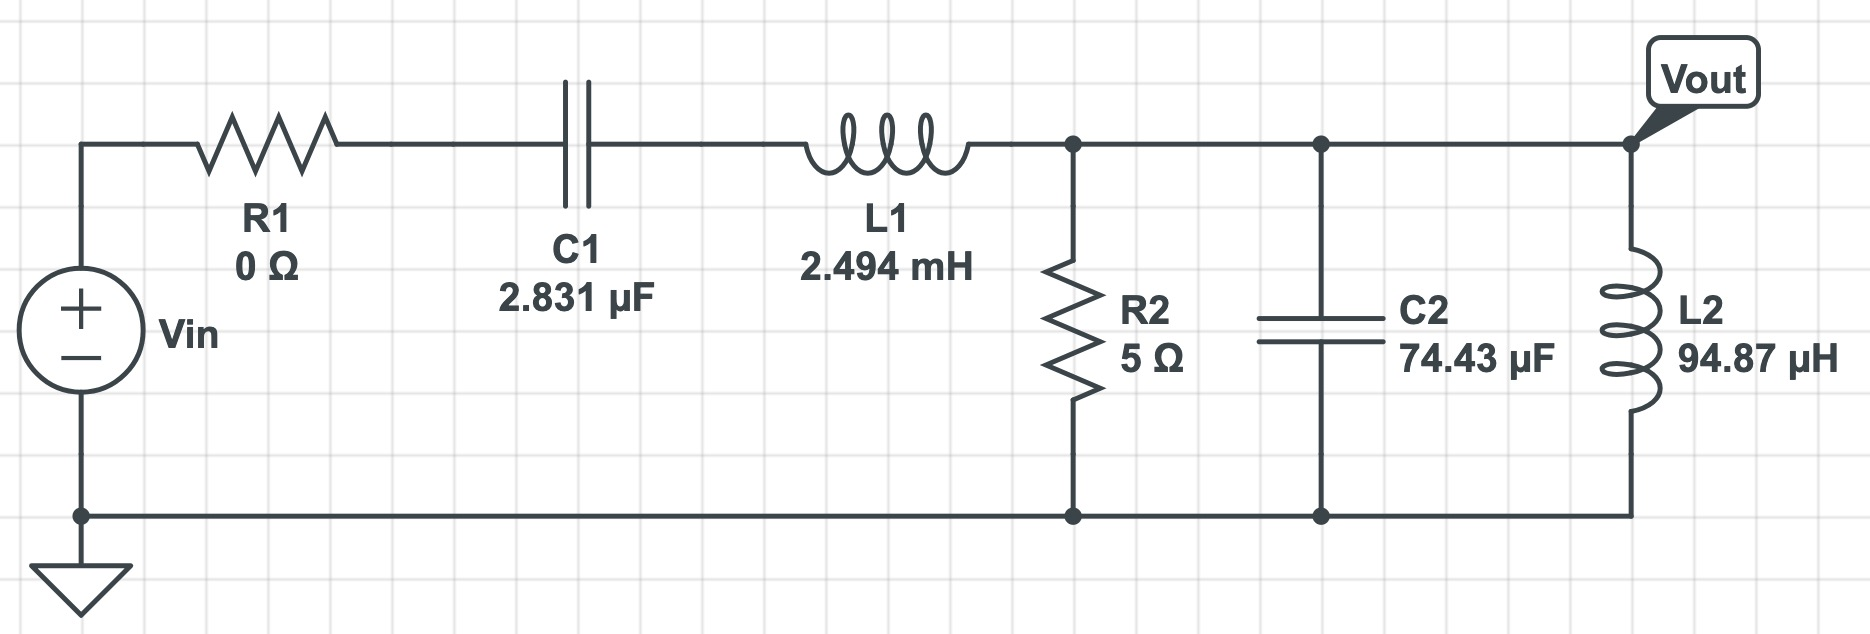
\includegraphics{Schematic.jpeg}
\caption{Filter Design}
\end{figure}

I started with arbitrary low values for the resistors, and then ran
simulations in LTSpice sweeping the values of both capacitors and
inductors. When the simulation showed reasonable attenuation for the 0
frequency range, as well as near 0.3 dB attenuation between 1800 and
2000 Hz, I used values nearer and nearer to those. This iterative
process took about an hour or so, but I ended up with the values shown
above.

Using this circuit, I derived the transfer function using the following
formula:

\[\frac{V_{in}-V_{out}}{R_1 + \frac{1}{sC_1}+sL_1}=\frac{V_{out}}{\frac{1}{sC_2}}+\frac{V_{out}}{sL_2}+\frac{V_{out}}{R_2}\]

Solving for \(V_{out}\)\ldots{}

\[V_{out}=\frac{s^2C_1L_2R_2V_{in}}{s^4C_1C_2L_1L_2R_2+s^3(C_1C_2L_2R_1R_2+C_1L_1L_2)+s^2(C_1L_1R_2+C_1L_2R_1+C_1L_2R_2+C_2L_2R_2)+s(L_2+C_1R_1R_2)+R_2}\]

\[H(s)=\frac{s^2C_1L_2R_2}{s^4C_1C_2L_1L_2R_2+s^3(C_1C_2L_2R_1R_2+C_1L_1L_2)+s^2(C_1L_1R_2+C_1L_2R_1+C_1L_2R_2+C_2L_2R_2)+s(L_2+C_1R_1R_2)+R_2}\]

\hypertarget{task-3}{%
\subsubsection{Task 3}\label{task-3}}

This transfer function's Bode plot can be plotted as follows:

    \begin{Verbatim}[commandchars=\\\{\}]
{\color{incolor}In [{\color{incolor}7}]:} \PY{n}{c1}\PY{p}{,} \PY{n}{c2} \PY{o}{=} \PY{l+m+mf}{2.831e\PYZhy{}6}\PY{p}{,} \PY{l+m+mf}{74.43e\PYZhy{}6}
        \PY{n}{l1}\PY{p}{,} \PY{n}{l2} \PY{o}{=} \PY{l+m+mf}{2.494e\PYZhy{}3}\PY{p}{,} \PY{l+m+mf}{94.87e\PYZhy{}6}
        \PY{n}{r1}\PY{p}{,} \PY{n}{r2} \PY{o}{=} \PY{l+m+mi}{0}\PY{p}{,} \PY{l+m+mi}{5}
        
        \PY{n}{num} \PY{o}{=} \PY{p}{[}\PY{n}{c1}\PY{o}{*}\PY{n}{l2}\PY{o}{*}\PY{n}{r2}\PY{p}{,} \PY{l+m+mi}{0}\PY{p}{,} \PY{l+m+mi}{0}\PY{p}{]}
        \PY{n}{den} \PY{o}{=} \PY{p}{[}\PY{n}{c1}\PY{o}{*}\PY{n}{c2}\PY{o}{*}\PY{n}{l1}\PY{o}{*}\PY{n}{l2}\PY{o}{*}\PY{n}{r2}\PY{p}{,} \PY{n}{c1}\PY{o}{*}\PY{n}{c2}\PY{o}{*}\PY{n}{l2}\PY{o}{*}\PY{n}{r1}\PY{o}{*}\PY{n}{r2}\PY{o}{+}\PY{n}{c1}\PY{o}{*}\PY{n}{l1}\PY{o}{*}\PY{n}{l2}\PY{p}{,}
               \PY{n}{c1}\PY{o}{*}\PY{n}{l1}\PY{o}{*}\PY{n}{r2}\PY{o}{+}\PY{n}{c1}\PY{o}{*}\PY{n}{l2}\PY{o}{*}\PY{n}{r1}\PY{o}{+}\PY{n}{c1}\PY{o}{*}\PY{n}{l2}\PY{o}{*}\PY{n}{r2}\PY{o}{+}\PY{n}{c2}\PY{o}{*}\PY{n}{l2}\PY{o}{*}\PY{n}{r2}\PY{p}{,} \PY{n}{l2}\PY{o}{+}\PY{n}{c1}\PY{o}{*}\PY{n}{r1}\PY{o}{*}\PY{n}{r2}\PY{p}{,} \PY{n}{r2}\PY{p}{]}
        \PY{n}{w} \PY{o}{=} \PY{n}{np}\PY{o}{.}\PY{n}{arange}\PY{p}{(}\PY{l+m+mi}{0}\PY{p}{,} \PY{l+m+mf}{1e6} \PY{o}{+} \PY{l+m+mi}{1}\PY{p}{,} \PY{l+m+mi}{1}\PY{p}{)}     \PY{c+c1}{\PYZsh{} Frequency in rad/s}
        \PY{n}{f} \PY{o}{=} \PY{p}{[}\PY{n}{v} \PY{o}{/} \PY{p}{(}\PY{l+m+mi}{2} \PY{o}{*} \PY{n}{np}\PY{o}{.}\PY{n}{pi}\PY{p}{)} \PY{k}{for} \PY{n}{v} \PY{o+ow}{in} \PY{n}{w}\PY{p}{]} \PY{c+c1}{\PYZsh{} Frequency in Hz}
        
        \PY{n}{plt}\PY{o}{.}\PY{n}{figure}\PY{p}{(}\PY{n}{figsize}\PY{o}{=}\PY{p}{(}\PY{l+m+mi}{16}\PY{p}{,} \PY{l+m+mi}{12}\PY{p}{)}\PY{p}{)}
        \PY{n}{system} \PY{o}{=} \PY{n}{control}\PY{o}{.}\PY{n}{TransferFunction}\PY{p}{(}\PY{n}{num}\PY{p}{,} \PY{n}{den}\PY{p}{)}
        \PY{n}{m}\PY{p}{,} \PY{n}{p}\PY{p}{,} \PY{n}{o} \PY{o}{=} \PY{n}{control}\PY{o}{.}\PY{n}{bode}\PY{p}{(}\PY{n}{system}\PY{p}{,} \PY{n}{w}\PY{p}{,} \PY{n}{dB}\PY{o}{=}\PY{k+kc}{True}\PY{p}{,} \PY{n}{Hz}\PY{o}{=}\PY{k+kc}{True}\PY{p}{,} \PY{n}{Plot}\PY{o}{=}\PY{k+kc}{True}\PY{p}{,} \PY{n}{deg}\PY{o}{=}\PY{k+kc}{True}\PY{p}{,} \PY{n}{color}\PY{o}{=}\PY{l+s+s1}{\PYZsq{}}\PY{l+s+s1}{r}\PY{l+s+s1}{\PYZsq{}}\PY{p}{)}
\end{Verbatim}

    \begin{center}
    \adjustimage{max size={0.9\linewidth}{0.9\paperheight}}{output_11_0.png}
    \end{center}
    { \hspace*{\fill} \\}
    
    To verify the filter specifications, because I cannot change the above
Bode-plot, I'll take a look at the provided frequency ranges, and look
at the magnitude of the filter's response over those ranges of
frequencies. This is all shown below, as well as plots of the filter's
response to those frequencies.

    \begin{Verbatim}[commandchars=\\\{\}]
{\color{incolor}In [{\color{incolor}8}]:} \PY{n}{pos\PYZus{}f}\PY{p}{,} \PY{n}{pos\PYZus{}m} \PY{o}{=} \PY{n}{subdivide\PYZus{}freq\PYZus{}mag}\PY{p}{(}\PY{n}{f}\PY{p}{,} \PY{n}{m}\PY{p}{,} \PY{p}{[}\PY{l+m+mi}{1750}\PY{p}{,} \PY{l+m+mi}{2050}\PY{p}{]}\PY{p}{)}
        \PY{n+nb}{print} \PY{p}{(}\PY{l+s+s2}{\PYZdq{}}\PY{l+s+s2}{The signal is at most attenuated by }\PY{l+s+si}{\PYZpc{}f}\PY{l+s+s2}{ dB.}\PY{l+s+s2}{\PYZdq{}} \PY{o}{\PYZpc{}} \PY{n+nb}{min}\PY{p}{(}\PY{n}{pos\PYZus{}m}\PY{p}{)}\PY{p}{)}
        
        \PY{n}{lowf\PYZus{}vib\PYZus{}f}\PY{p}{,} \PY{n}{lowf\PYZus{}vib\PYZus{}m} \PY{o}{=} \PY{n}{subdivide\PYZus{}freq\PYZus{}mag}\PY{p}{(}\PY{n}{f}\PY{p}{,} \PY{n}{m}\PY{p}{,} \PY{p}{[}\PY{l+m+mi}{15000}\PY{p}{,} \PY{l+m+mi}{30000}\PY{p}{]}\PY{p}{)}
        \PY{n+nb}{print} \PY{p}{(}\PY{l+s+s2}{\PYZdq{}}\PY{l+s+s2}{The low\PYZhy{}frequency vibration noise is attenuated by at least }\PY{l+s+si}{\PYZpc{}f}\PY{l+s+s2}{ dB.}\PY{l+s+s2}{\PYZdq{}}
               \PY{o}{\PYZpc{}} \PY{n+nb}{max}\PY{p}{(}\PY{n}{lowf\PYZus{}vib\PYZus{}m}\PY{p}{)}\PY{p}{)}
        
        \PY{n}{switch\PYZus{}f}\PY{p}{,} \PY{n}{switch\PYZus{}m} \PY{o}{=} \PY{n}{subdivide\PYZus{}freq\PYZus{}mag}\PY{p}{(}\PY{n}{f}\PY{p}{,} \PY{n}{m}\PY{p}{,} \PY{p}{[}\PY{l+m+mi}{75000}\PY{p}{,} \PY{l+m+mi}{100000}\PY{p}{]}\PY{p}{)}
        \PY{n+nb}{print} \PY{p}{(}\PY{l+s+s2}{\PYZdq{}}\PY{l+s+s2}{The switching\PYZhy{}amplifier noise is attenuated by at least }\PY{l+s+si}{\PYZpc{}f}\PY{l+s+s2}{ dB.}\PY{l+s+s2}{\PYZdq{}}
               \PY{o}{\PYZpc{}} \PY{n+nb}{max}\PY{p}{(}\PY{n}{switch\PYZus{}m}\PY{p}{)}\PY{p}{)}
        
        \PY{n}{highf\PYZus{}noise\PYZus{}f}\PY{p}{,} \PY{n}{highf\PYZus{}noise\PYZus{}m} \PY{o}{=} \PY{n}{subdivide\PYZus{}freq\PYZus{}mag}\PY{p}{(}\PY{n}{f}\PY{p}{,} \PY{n}{m}\PY{p}{,} \PY{p}{[}\PY{l+m+mi}{100000}\PY{p}{,} \PY{n+nb}{max}\PY{p}{(}\PY{n}{f}\PY{p}{)}\PY{p}{]}\PY{p}{)}
        \PY{n+nb}{print} \PY{p}{(}\PY{l+s+s2}{\PYZdq{}}\PY{l+s+s2}{All noises higher than 100 kHz are attenuated by at least }\PY{l+s+si}{\PYZpc{}f}\PY{l+s+s2}{ dB.}\PY{l+s+s2}{\PYZdq{}}
               \PY{o}{\PYZpc{}} \PY{n+nb}{max}\PY{p}{(}\PY{n}{highf\PYZus{}noise\PYZus{}m}\PY{p}{)}\PY{p}{)}
\end{Verbatim}

    \begin{Verbatim}[commandchars=\\\{\}]
The signal is at most attenuated by -0.000001 dB.
The low-frequency vibration noise is attenuated by at least -64.062774 dB.
The switching-amplifier noise is attenuated by at least -92.291386 dB.
All noises higher than 100 kHz are attenuated by at least -97.293825 dB.

    \end{Verbatim}

    \begin{Verbatim}[commandchars=\\\{\}]
{\color{incolor}In [{\color{incolor}9}]:} \PY{n}{create\PYZus{}plot}\PY{p}{(}\PY{p}{[}\PY{n}{pos\PYZus{}f}\PY{p}{,} \PY{n}{lowf\PYZus{}vib\PYZus{}f}\PY{p}{,} \PY{n}{switch\PYZus{}f}\PY{p}{,} \PY{n}{highf\PYZus{}noise\PYZus{}f}\PY{p}{]}\PY{p}{,}
                    \PY{p}{[}\PY{p}{(}\PY{n}{pos\PYZus{}m}\PY{p}{,} \PY{p}{)}\PY{p}{,} \PY{p}{(}\PY{n}{lowf\PYZus{}vib\PYZus{}m}\PY{p}{,} \PY{p}{)}\PY{p}{,} \PY{p}{(}\PY{n}{switch\PYZus{}m}\PY{p}{,} \PY{p}{)}\PY{p}{,} \PY{p}{(}\PY{n}{highf\PYZus{}noise\PYZus{}m}\PY{p}{,} \PY{p}{)}\PY{p}{]}\PY{p}{,}
                    \PY{p}{[}\PY{l+s+s2}{\PYZdq{}}\PY{l+s+s2}{Frequency (Hz)}\PY{l+s+s2}{\PYZdq{}}\PY{p}{,} \PY{l+s+s2}{\PYZdq{}}\PY{l+s+s2}{Frequency (Hz)}\PY{l+s+s2}{\PYZdq{}}\PY{p}{,} \PY{l+s+s2}{\PYZdq{}}\PY{l+s+s2}{Frequency (Hz)}\PY{l+s+s2}{\PYZdq{}}\PY{p}{,} \PY{l+s+s2}{\PYZdq{}}\PY{l+s+s2}{Frequency (Hz)}\PY{l+s+s2}{\PYZdq{}}\PY{p}{]}\PY{p}{,}
                    \PY{p}{[}\PY{l+s+s2}{\PYZdq{}}\PY{l+s+s2}{Magnitude (dB)}\PY{l+s+s2}{\PYZdq{}}\PY{p}{,} \PY{l+s+s2}{\PYZdq{}}\PY{l+s+s2}{Magnitude (dB)}\PY{l+s+s2}{\PYZdq{}}\PY{p}{,} \PY{l+s+s2}{\PYZdq{}}\PY{l+s+s2}{Magnitude (dB)}\PY{l+s+s2}{\PYZdq{}}\PY{p}{,} \PY{l+s+s2}{\PYZdq{}}\PY{l+s+s2}{Magnitude (dB)}\PY{l+s+s2}{\PYZdq{}}\PY{p}{]}\PY{p}{,}
                    \PY{p}{[}\PY{p}{(}\PY{l+s+s2}{\PYZdq{}}\PY{l+s+s2}{Attenuation of the position sensor}\PY{l+s+s2}{\PYZdq{}}\PY{p}{,} \PY{p}{)}\PY{p}{,}
                     \PY{p}{(}\PY{l+s+s2}{\PYZdq{}}\PY{l+s+s2}{Attenuation of the low\PYZhy{}frequency vibration}\PY{l+s+s2}{\PYZdq{}}\PY{p}{,} \PY{p}{)}\PY{p}{,}
                     \PY{p}{(}\PY{l+s+s2}{\PYZdq{}}\PY{l+s+s2}{Attenuation of the switching\PYZhy{}amplifier noise}\PY{l+s+s2}{\PYZdq{}}\PY{p}{,} \PY{p}{)}\PY{p}{,}
                     \PY{p}{(}\PY{l+s+s2}{\PYZdq{}}\PY{l+s+s2}{Attenuation of all frequencies greater than 100 kHz}\PY{l+s+s2}{\PYZdq{}}\PY{p}{,} \PY{p}{)}\PY{p}{]}\PY{p}{,}
                    \PY{n}{mode\PYZus{}list}\PY{o}{=}\PY{p}{[}\PY{l+s+s2}{\PYZdq{}}\PY{l+s+s2}{Log}\PY{l+s+s2}{\PYZdq{}}\PY{p}{,} \PY{l+s+s2}{\PYZdq{}}\PY{l+s+s2}{Log}\PY{l+s+s2}{\PYZdq{}}\PY{p}{,} \PY{l+s+s2}{\PYZdq{}}\PY{l+s+s2}{Log}\PY{l+s+s2}{\PYZdq{}}\PY{p}{,} \PY{l+s+s2}{\PYZdq{}}\PY{l+s+s2}{Log}\PY{l+s+s2}{\PYZdq{}}\PY{p}{]}\PY{p}{,} \PY{n}{num\PYZus{}rows}\PY{o}{=}\PY{l+m+mi}{4}\PY{p}{)}
\end{Verbatim}

    \begin{center}
    \adjustimage{max size={0.9\linewidth}{0.9\paperheight}}{output_14_0.png}
    \end{center}
    { \hspace*{\fill} \\}
    
    \hypertarget{task-4}{%
\subsubsection{Task 4}\label{task-4}}

Now, to pass the input signal through my above-defined filter. Based off
the information of the Bode-plot of my filter, and the FFT results of my
input signal, I expect all the high-frequency noise to be removed, and
the remaining signal to be solely comprised of signals between the
frequency range of 1800 and 2000 Hz.

    \begin{Verbatim}[commandchars=\\\{\}]
{\color{incolor}In [{\color{incolor}10}]:} \PY{c+c1}{\PYZsh{} Pass the input signal through the filter}
         \PY{n}{z\PYZus{}num}\PY{p}{,} \PY{n}{z\PYZus{}den} \PY{o}{=} \PY{n}{signal}\PY{o}{.}\PY{n}{bilinear}\PY{p}{(}\PY{n}{num}\PY{p}{,} \PY{n}{den}\PY{p}{,} \PY{n}{f\PYZus{}samp}\PY{p}{)}
         \PY{n}{filt}  \PY{o}{=} \PY{n}{signal}\PY{o}{.}\PY{n}{lfilter}\PY{p}{(}\PY{n}{z\PYZus{}num}\PY{p}{,} \PY{n}{z\PYZus{}den}\PY{p}{,} \PY{n}{sensor\PYZus{}sig}\PY{p}{)}
         \PY{n}{create\PYZus{}plot}\PY{p}{(}\PY{p}{[}\PY{n}{t}\PY{p}{,} \PY{n}{t}\PY{p}{]}\PY{p}{,} \PY{p}{[}\PY{p}{(}\PY{n}{sensor\PYZus{}sig}\PY{p}{,} \PY{p}{)}\PY{p}{,} \PY{p}{(}\PY{n}{filt}\PY{p}{,} \PY{p}{)}\PY{p}{]}\PY{p}{,}
                     \PY{p}{[}\PY{l+s+s2}{\PYZdq{}}\PY{l+s+s2}{t (s)}\PY{l+s+s2}{\PYZdq{}}\PY{p}{,} \PY{l+s+s2}{\PYZdq{}}\PY{l+s+s2}{t (s)}\PY{l+s+s2}{\PYZdq{}}\PY{p}{]}\PY{p}{,} \PY{p}{[}\PY{l+s+s2}{\PYZdq{}}\PY{l+s+s2}{\PYZdl{}y(t)\PYZdl{}}\PY{l+s+s2}{\PYZdq{}}\PY{p}{,} \PY{l+s+s2}{\PYZdq{}}\PY{l+s+s2}{\PYZdl{}y(t)\PYZdl{}}\PY{l+s+s2}{\PYZdq{}}\PY{p}{]}\PY{p}{,}
                     \PY{p}{[}\PY{p}{(}\PY{l+s+s2}{\PYZdq{}}\PY{l+s+s2}{Original Function}\PY{l+s+s2}{\PYZdq{}}\PY{p}{,} \PY{p}{)}\PY{p}{,} \PY{p}{(}\PY{l+s+s2}{\PYZdq{}}\PY{l+s+s2}{Filtered Function}\PY{l+s+s2}{\PYZdq{}}\PY{p}{,} \PY{p}{)}\PY{p}{]}\PY{p}{,}
                     \PY{n}{mode\PYZus{}list}\PY{o}{=}\PY{p}{[}\PY{l+s+s2}{\PYZdq{}}\PY{l+s+s2}{Norm}\PY{l+s+s2}{\PYZdq{}}\PY{p}{,} \PY{l+s+s2}{\PYZdq{}}\PY{l+s+s2}{Norm}\PY{l+s+s2}{\PYZdq{}}\PY{p}{]}\PY{p}{,} \PY{n}{num\PYZus{}rows}\PY{o}{=}\PY{l+m+mi}{2}\PY{p}{)}
\end{Verbatim}

    \begin{center}
    \adjustimage{max size={0.9\linewidth}{0.9\paperheight}}{output_16_0.png}
    \end{center}
    { \hspace*{\fill} \\}
    
    The results of this filter can be verified in two additional ways. I'll
compute the FFT analysis of the filtered signal, and all the results (of
significant magnitude) should lie in the sensor's frequency range. In
addition to this, I'll visually compare the filtered signal to a signal
of 1900 Hz, to visually compare the two's frequency (as amplitude does
not matter).

    \begin{Verbatim}[commandchars=\\\{\}]
{\color{incolor}In [{\color{incolor}12}]:} \PY{c+c1}{\PYZsh{} Compute the FFT of the filtered signal}
         \PY{n}{filt\PYZus{}fft\PYZus{}freq}\PY{p}{,} \PY{n}{filt\PYZus{}x\PYZus{}mag}\PY{p}{,} \PY{n}{\PYZus{}} \PY{o}{=} \PY{n}{fast\PYZus{}fourier}\PY{p}{(}\PY{n}{filt}\PY{p}{,} \PY{n}{f\PYZus{}samp}\PY{p}{)}
         \PY{c+c1}{\PYZsh{} Ignore the negative frequencies}
         \PY{n}{filt\PYZus{}fft\PYZus{}freq} \PY{o}{=} \PY{n}{filt\PYZus{}fft\PYZus{}freq}\PY{p}{[}\PY{p}{:}\PY{n+nb}{len}\PY{p}{(}\PY{n}{filt\PYZus{}fft\PYZus{}freq}\PY{p}{)}\PY{o}{/}\PY{o}{/}\PY{l+m+mi}{2}\PY{p}{]}
         \PY{n}{filt\PYZus{}x\PYZus{}mag}    \PY{o}{=} \PY{n}{filt\PYZus{}x\PYZus{}mag}\PY{p}{[}\PY{p}{:}\PY{n+nb}{len}\PY{p}{(}\PY{n}{filt\PYZus{}x\PYZus{}mag}\PY{p}{)}\PY{o}{/}\PY{o}{/}\PY{l+m+mi}{2}\PY{p}{]}
         \PY{n}{sub\PYZus{}freq}\PY{p}{,} \PY{n}{sub\PYZus{}mag} \PY{o}{=} \PY{n}{subdivide\PYZus{}freq\PYZus{}mag}\PY{p}{(}\PY{n}{filt\PYZus{}fft\PYZus{}freq}\PY{p}{,} \PY{n}{filt\PYZus{}x\PYZus{}mag}\PY{p}{,} \PY{p}{[}\PY{l+m+mi}{1500}\PY{p}{,} \PY{l+m+mi}{2500}\PY{p}{]}\PY{p}{,} \PY{n}{mode}\PY{o}{=}\PY{l+s+s2}{\PYZdq{}}\PY{l+s+s2}{Norm}\PY{l+s+s2}{\PYZdq{}}\PY{p}{)}
         
         \PY{n}{create\PYZus{}plot}\PY{p}{(}\PY{p}{[}\PY{n}{filt\PYZus{}fft\PYZus{}freq}\PY{p}{,} \PY{n}{sub\PYZus{}freq}\PY{p}{,} \PY{n}{t}\PY{p}{]}\PY{p}{,}
                     \PY{p}{[}\PY{p}{(}\PY{n}{filt\PYZus{}x\PYZus{}mag}\PY{p}{,} \PY{p}{)}\PY{p}{,} \PY{p}{(}\PY{n}{sub\PYZus{}mag}\PY{p}{,} \PY{p}{)}\PY{p}{,} \PY{p}{(}\PY{n}{filt}\PY{p}{,} \PY{l+m+mf}{2.5}\PY{o}{*}\PY{n}{np}\PY{o}{.}\PY{n}{cos}\PY{p}{(}\PY{l+m+mi}{2} \PY{o}{*} \PY{n}{np}\PY{o}{.}\PY{n}{pi} \PY{o}{*} \PY{l+m+mi}{1900} \PY{o}{*} \PY{n}{t}\PY{p}{)}\PY{p}{)}\PY{p}{]}\PY{p}{,}
                     \PY{p}{[}\PY{l+s+s2}{\PYZdq{}}\PY{l+s+s2}{\PYZdl{}f\PYZdl{}}\PY{l+s+s2}{\PYZdq{}}\PY{p}{,} \PY{l+s+s2}{\PYZdq{}}\PY{l+s+s2}{\PYZdl{}f}\PY{l+s+s2}{\PYZdq{}}\PY{p}{,} \PY{l+s+s2}{\PYZdq{}}\PY{l+s+s2}{\PYZdl{}t\PYZdl{}}\PY{l+s+s2}{\PYZdq{}}\PY{p}{]}\PY{p}{,}
                     \PY{p}{[}\PY{l+s+s2}{\PYZdq{}}\PY{l+s+s2}{Magnitude of FFT(x(t))}\PY{l+s+s2}{\PYZdq{}}\PY{p}{,} \PY{l+s+s2}{\PYZdq{}}\PY{l+s+s2}{Magnitude of FFT(x(t))}\PY{l+s+s2}{\PYZdq{}}\PY{p}{,} \PY{l+s+s2}{\PYZdq{}}\PY{l+s+s2}{Amplitude (V)}\PY{l+s+s2}{\PYZdq{}}\PY{p}{]}\PY{p}{,}
                     \PY{p}{[}\PY{p}{(}\PY{l+s+s2}{\PYZdq{}}\PY{l+s+s2}{\PYZdl{}|FFT(x(t))|\PYZdl{} of all frequencies}\PY{l+s+s2}{\PYZdq{}}\PY{p}{,} \PY{p}{)}\PY{p}{,}
                      \PY{p}{(}\PY{l+s+s2}{\PYZdq{}}\PY{l+s+s2}{\PYZdl{}|FFT(x(t))|\PYZdl{} of just the sensor frequencies}\PY{l+s+s2}{\PYZdq{}}\PY{p}{,} \PY{p}{)}\PY{p}{,}
                      \PY{p}{(}\PY{l+s+s2}{\PYZdq{}}\PY{l+s+s2}{Filtered \PYZdl{}x(t)\PYZdl{}}\PY{l+s+s2}{\PYZdq{}}\PY{p}{,} \PY{l+s+s2}{\PYZdq{}}\PY{l+s+s2}{Comparison 1,900 Hz Cosine Function}\PY{l+s+s2}{\PYZdq{}}\PY{p}{)}\PY{p}{]}\PY{p}{,}
                     \PY{p}{[}\PY{l+s+s2}{\PYZdq{}}\PY{l+s+s2}{Stem}\PY{l+s+s2}{\PYZdq{}}\PY{p}{,} \PY{l+s+s2}{\PYZdq{}}\PY{l+s+s2}{Stem}\PY{l+s+s2}{\PYZdq{}}\PY{p}{,} \PY{l+s+s2}{\PYZdq{}}\PY{l+s+s2}{Norm}\PY{l+s+s2}{\PYZdq{}}\PY{p}{]}\PY{p}{,} \PY{l+m+mi}{3}\PY{p}{)}
\end{Verbatim}

    \begin{center}
    \adjustimage{max size={0.9\linewidth}{0.9\paperheight}}{output_18_0.png}
    \end{center}
    { \hspace*{\fill} \\}
    
    The first two plots show the effect of the filtering on the signal.
Beforehand, many frequencies mixed with the sensor's output to create a
very messy signal. Clearly, all high-frequencies from other noise
sources are almost completely attenuated (as close to zero as possible).
The second plot is a zoomed in region from 1,500 Hz to 2,500 Hz. Because
the filter isn't perfect, you can see there is some remaining signals
outside the sensor's 1,800-2,000 Hz range, but their magnitude is very
small. Finally, the filtered signal is compared to a `normal' 1,900 Hz
cosine function in the final plot, just to visually show how the
remaining signal is clearly a very similar frequency (although not
exactly 1900, as shown in the fourier series in plot 2).

\hypertarget{questions}{%
\subsection{Questions}\label{questions}}

I feel as though there was plenty of labwork on analyzing filters, so I
felt adequately prepared for that portion of this final project.
However, we never did any labwork on the filter \emph{design} itself;
which meant I felt somewhat confused on where to start. Perhaps have a
lab on the \texttt{scipy.butter()} function, or any other filtering
functions available in the \texttt{SciPy} package. Other than that, I
felt as though the identification of the sampling frequency was a bit
confusing and arbitrary, and could drastically change the results of the
Fourier Transform. I ended up going with a relatively high sampling
frequency, but when I was testing with lower frequency sample rates my
results were drastically different (as expected).

\hypertarget{conclusion}{%
\subsection{Conclusion}\label{conclusion}}

This final project was very effective at re-applying the skills learned
throughout this semester of lab-work. Having a much more open-ended
problem meant that a lot of my work had to be `\emph{figured out}'
incrementally, rather than being given a step-by-step walkthrough for
the tasks required. Overall, I am very happy with the results of my
work. The filtered signal is \textbf{far} cleaner than the original
input signal, and the bode-plot of the filter fits exactly with the
design requirements.


    % Add a bibliography block to the postdoc
    
    
    
    \end{document}
